\documentclass[12pt, a4paper]{article}
\usepackage{tikz}
\usepackage{graphicx}
\usepackage{booktabs}
\usepackage{geometry}
\usepackage{float}
\usepackage{hyperref}
\geometry{margin=1in}

\title{Software Design and Architecture: \\ Pong Game Refactoring Evolution}
\author{}
\date{\today}

\begin{document}
\maketitle

\tableofcontents
\newpage

\section{Use Case Diagram and Scenarios}

\subsection{Use Case Diagram}
The following diagram illustrates the active users and the system use cases.
\vspace{1em}
\begin{figure}[H]
    \centering
    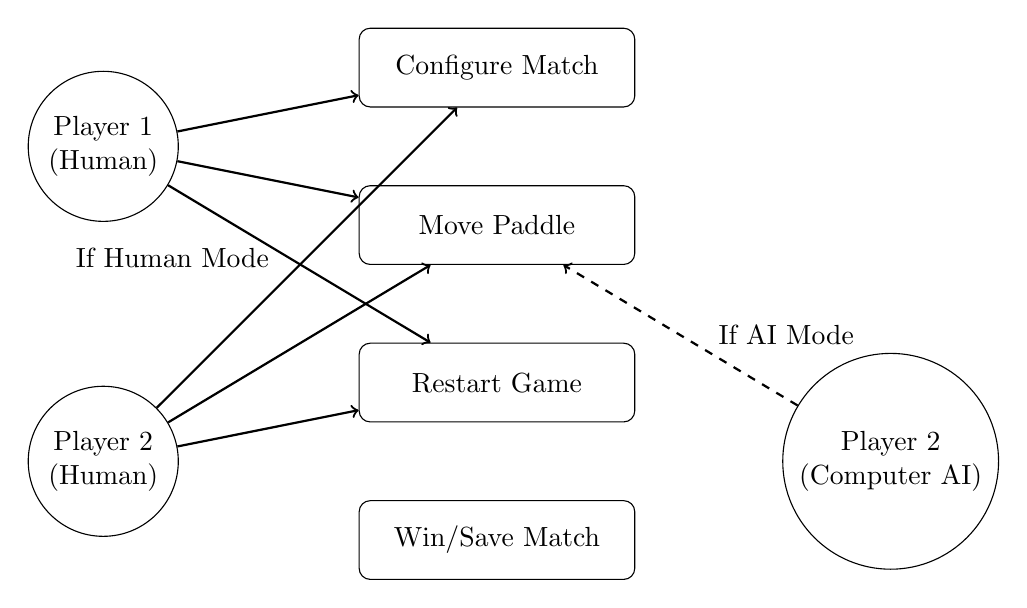
\begin{tikzpicture}
        % Actors
        \node[circle, draw, minimum size=1.5cm, align=center] (p1) at (0, 4) {Player 1 \\ (Human)};
        \node[circle, draw, minimum size=1.5cm, align=center] (p2) at (0, 0) {Player 2 \\ (Human)};
        \node[circle, draw, minimum size=1.5cm, align=center] (ai) at (10, 0) {Player 2 \\ (Computer AI)};
        
        % Use Cases
        \node[draw, rounded corners, minimum width=3.5cm, minimum height=1cm] (uc1) at (5, 5) {Configure Match};
        \node[draw, rounded corners, minimum width=3.5cm, minimum height=1cm] (uc2) at (5, 3) {Move Paddle};
        \node[draw, rounded corners, minimum width=3.5cm, minimum height=1cm] (uc3) at (5, 1) {Restart Game};
        \node[draw, rounded corners, minimum width=3.5cm, minimum height=1cm] (uc4) at (5, -1) {Win/Save Match};
        
        % Connections
        \draw[->, thick] (p1) -- (uc1);
        \draw[->, thick] (p1) -- (uc2);
        \draw[->, thick] (p1) -- (uc3);
        
        \draw[->, thick] (p2) -- (uc1) node[midway, left, xshift=-10pt] {If Human Mode};
        \draw[->, thick] (p2) -- (uc2);
        \draw[->, thick] (p2) -- (uc3);
        
        \draw[->, dashed, thick] (ai) -- (uc2) node[midway, right, xshift=10pt] {If AI Mode};
    \end{tikzpicture}
    \caption{System Use Case Diagram}
\end{figure}

\subsection{Use Case Scenarios}

\subsubsection*{UC1: Configure Match}
\textbf{Actors:} Player 1, Player 2 \\
\textbf{Preconditions:} The application is launched and the main window is visible. \\
\textbf{Main Flow:}
\begin{enumerate}
    \item System prompts: \textit{"Play against Computer? (Yes/No)"}.
    \item User inputs selection. If 'Yes', AI Mode is enabled.
    \item System prompts for Player 1 Name.
    \item System prompts for Player 2 Name (Skipped and defaulted to "Computer" if AI Mode is on).
    \item System prompts for Maximum Winning Score.
    \item Match initializes and the game loop starts.
\end{enumerate}

\subsubsection*{UC2: Move Paddle}
\textbf{Actors:} Player 1, Player 2 / Computer AI \\
\textbf{Preconditions:} Match is configured and runtime loop is active. \\
\textbf{Main Flow:}
\begin{enumerate}
    \item The Game Engine's \texttt{updateTick()} requests the next directional inputs.
    \item System polls the \texttt{IInputHandler}.
    \item Player 1 presses W/S keys; system assigns Player 1's paddle displacement.
    \item In Human Mode, Player 2 presses Up/Down keys. In AI Mode, the \texttt{AiInputHandler} intercepts the request, inspecting the exact Y-coordinates of the Ball and computing an automatic intercept vector.
    \item The system updates both paddles and the ball positions inside the \texttt{GameState}.
    \item Frame finishes and is sent to the Renderer.
\end{enumerate}

\subsubsection*{UC3: Win and Save Match}
\textbf{Actors:} System \\
\textbf{Preconditions:} The ball moves logically past the X-bound of either left or right paddles. \\
\textbf{Main Flow:}
\begin{enumerate}
    \item System detects goal scored and increments the opposing player's \texttt{PaddleModel} score.
    \item System checks if the new score equals or exceeds the Maximum Score limit.
    \item The Game Engine suspends the runtime loop.
    \item System delegates the final stats to the \texttt{CsvScoreRepository}.
    \item Data is appended asynchronously to \texttt{match\_results.csv}.
    \item System alerts the \texttt{IRenderer} to throw a modal announcing the winner to the user.
    \item System resets state and transitions back to Configure Match (UC1) seamlessly.
\end{enumerate}

\newpage
\section{Class Diagram Evolution}

\subsection{Original Version (Basic Architecture)}
The initial implementation suffered from the "God Class" anti-pattern and tight coupling to Java AWT graphics libraries. Dependencies were highly circular.

\begin{verbatim}
+-------------------+       +-------------------+
|      Window       |<>---->|       Game        |
+-------------------+       +-------------------+
                            | - ball: Ball      |
                            | - p1: Paddle      |
                            | - p2: Paddle      |
                            +-------------------+
                            | + run()           |
                            | + draw(Graphics)  |
                            | + update()        |
                            | + setupGame()     |
                            +-------------------+
                               /      |      \
                              /       |       \
                             v        v        v
        +-------------------+  +---------------+  +--------------+
        |     KeyInput      |  |     Ball      |  |    Paddle    |
        +-------------------+  +---------------+  +--------------+
        | - p1: Paddle      |  | + draw(G)     |  | + draw(G)    |
        | - p2: Paddle      |  | + update()    |  | + update()   |
        +-------------------+  +---------------+  +--------------+
\end{verbatim}

\vspace{2em}
\subsection{Current Refactored Version (MVC + Strategy + Decorator Pattern)}
The new architecture strictly separates the Model, View, Controller, and Data Access layers via Interfaces, resulting in a loosely coupled and highly testable design.

\begin{verbatim}
=============================================================================
[ INTERFACES ] (Contracts defining behavior regardless of platform)
=============================================================================
 <<IRenderer>>         <<IInputHandler>>          <<IScoreRepository>>

=============================================================================
[ CONTROLLERS ] (Logic Engine and Orchestrators)
=============================================================================
 + GameEngine (Runnable)
     -- Orchestrates interactions using exclusively Interfaces.
 + AiInputHandler (implements IInputHandler)
     -- Decorator pattern wrapping around human input logic for P2.

=============================================================================
[ MODELS ] (Pure State logic, Zero Graphics/AWT dependencies)
=============================================================================
 + GameState 
     -- Manages global bounds, constraints, and holds component classes.
 + BallModel
 + PaddleModel

=============================================================================
[ UI / PRESENTATION ] (Concrete Swing implementation of Interfaces)
=============================================================================
 + SwingGamePanel (implements IRenderer)
 + SwingKeyInput (implements IInputHandler)
 + GameWindow (JFrame Wrapper)

=============================================================================
[ DATA ACCESS ] 
=============================================================================
 + CsvScoreRepository (implements IScoreRepository)
\end{verbatim}

\newpage
\section{Sequence Diagram}

The following textual sequence details the runtime execution loop (a single tick) showcasing the Decorator Pattern intercepting the input generation when AI Mode is selected.

\vspace{1em}
\begin{verbatim}
Title: Frame Update Tick (AI Mode Enabled)

// 1. Controller Polls for Player 1 Input
GameEngine -> AiInputHandler: getPlayer1Direction()
AiInputHandler -> SwingKeyInput: getPlayer1Direction()
SwingKeyInput --> AiInputHandler: return direction (human key pressed)
AiInputHandler --> GameEngine: return p1Direction

// 2. Controller Polls for Player 2 Input
GameEngine -> AiInputHandler: getPlayer2Direction()
AiInputHandler -> GameState: getBall().getY()
GameState --> AiInputHandler: return ballY
AiInputHandler -> GameState: getRightPaddle().getY()
GameState --> AiInputHandler: return paddleY
Note right of AiInputHandler: Performs tracking/intercept calculus
AiInputHandler --> GameEngine: return calculated p2Direction

// 3. Controller applies calculated inputs to the Model
GameEngine -> GameState: update(p1Direction, p2Direction)
GameState -> PaddleModel: updatePosition()
GameState -> BallModel: update()
GameState -> GameState: checkCollisions()
GameState --> GameEngine: update complete

// 4. Controller checks victory states
GameEngine -> GameState: checkWin()
GameState --> GameEngine: return null (signifying game is still running)

// 5. Controller alerts standard View layer
GameEngine -> SwingGamePanel: renderFrame(GameState)
SwingGamePanel -> GameState: get active properties
SwingGamePanel -> Screen: Paint with AWT / Graphics
SwingGamePanel --> GameEngine: Draw complete
\end{verbatim}

\end{document}
